\documentclass[11pt,a4paper]{article}
\usepackage{amsmath,verbatim}
\usepackage{listings}
\usepackage[english]{babel}
%\usepackage{movie15}
\usepackage{multimedia}
\usepackage{graphicx}
\usepackage{url}
\newcommand{\Deltap}{\ensuremath{\Delta^{\!+}}}
\newcommand{\trans}{\ensuremath{{}^\mathrm{T}}}
\newcommand{\eps}{\varepsilon}
\newcommand*{\approxdist}{\mathrel{\vcenter{\offinterlineskip
\vskip-.25ex\hbox{\hskip.55ex$\cdot$}\vskip-.25ex\hbox{$\sim$}
\vskip-.5ex\hbox{\hskip.55ex$\cdot$}}}}

% \lstMakeShortInline[language=myR]¬

\lstdefinelanguage{myR}
{
   language=R,
   otherkeywords={read.table, set.seed, head},
   deletekeywords={url,codes, t, dt, Call, formula,Q, R, on,by,hat,is,
col, set,start,end,deltat,zip},
   sensitive=true,
   breaklines=true,
   morecomment=[l]{\#},
   morestring=[b]",
   morestring=[b]',
   basicstyle =\ttfamily\small,
   keywordstyle=\bfseries,
   showtabs=false,
   showstringspaces=false,
   literate= {~}{$\sim$}{2},
   numberstyle=\sffamily\scriptsize,
   stepnumber=2
 }

\oddsidemargin=-0.4in
\evensidemargin=-0.4in
\topmargin=-0.5in
\textheight=9.5in
\textwidth=7in

\title{Discussion of: Unbiased MCMC with couplings (Jacob \emph{et al})}
\author{Darren J.\ Wilkinson}
\date{Newcastle University}

\begin{document}

\maketitle

The authors are to be congratulated for this interesting and useful contribution to the Markov chain Monte Carlo (MCMC) literature. Since in general we cannot initialise an MCMC chain with an exact sample from the target, we rely on asymptotic convergence to equilibrium, but lack of convergence leads to biased estimates.
The method outlined in the paper provides a method for removing the bias from any estimates that are produced from the algorithm output, by using a pair of coupled chains.
The approach is quite general, and can potentially be applied to many different kinds of MCMC algorithms --- this paper concentrates on Metropolis--Hastings and Gibbs sampling, but there are several related papers exploring applications to other MCMC schemes. 

It is important to keep in mind that coalescence of the coupled chains and convergence to equilibrium are different. Practical application of the method relies on the
time-averaged estimator (equation 2.1 in the paper).
This is just the regular MCMC estimate with a correction term that terminates once the chains have coupled. Choosing $k$ (the ``burn-in'') to be a high quantile of the coupling-time distribution will ensure that most estimates contain no correction at all. But since $k$ represents ``wasted'' computation, it seems desirable to encourage the chains to couple rapidly. Although it is possible to engineer early coupling (via identical initial conditions and a low-acceptance rate Metropolis--Hastings kernel, for example), this might be a dangerous strategy (see example 5.1 in the paper). When the correction term is present, it can sometimes be large, so developing a better understanding the distributional properties of the correction term is likely to be useful.

The technique proposed for coupling Metropolis--Hastings kernels works for multivariate as well as univariate samplers, though reflection maximal coupling works much better than a simple independent maximal coupling in high dimensions. However, it also makes sense to want to couple Gibbs samplers and other component-wise update algorithms. The paper proposes that for each component update of a Gibbs sampler, the full-conditionals for the two chains should be coupled. It is clear that once all components have coalesced, the full state of the chain will match, and the coupling of the two chains will be faithful. There is little theory providing reassurance that this will happen in reasonable time for challenging problems, though it does seem to work reasonably well, empirically.
  
Consider a linear Gaussian AR(1) process defined by
$$
X_t = \alpha X_{t-1} + \epsilon_t,\qquad \epsilon_t \sim {\mathrm N}(0,\sigma^2),
$$
for $t=1,2,\ldots,T$, with periodic boundaries. The full-conditional for each variable $X_t$ is of the form
$$
X_t|X_{t-1},X_{t+1} \sim {\mathrm N}\left(\frac{\alpha}{1+\alpha^2}(X_{t-1}+X_{t+1}), \frac{\sigma^2}{1+\alpha^2} \right).
$$
We can run two chains by cycling through each variable in turn and sampling from the coupled full conditionals. Here we use $T=200$ and $\alpha=0.99$, and run initially for $n=500$ iterations. By studying the coupling of variables in the Gibbs sampler, we see that coupling follows a stochastic process, somewhat reminiscent of the annealing of a 1-d Ising model, and that it is not always rapid. We can study the coupling time distribution for this model with simple Monte Carlo, in order to find that the mean coupling time is around 2.6K, with a median of around 1K. The distribution is long-tailed, with a maximum observed coupling time over 1K replicates of 67K. Choosing $k$ to be a very high quantile of this distribution will therefore be computationally demanding.

\begin{figure}
  \centerline{
    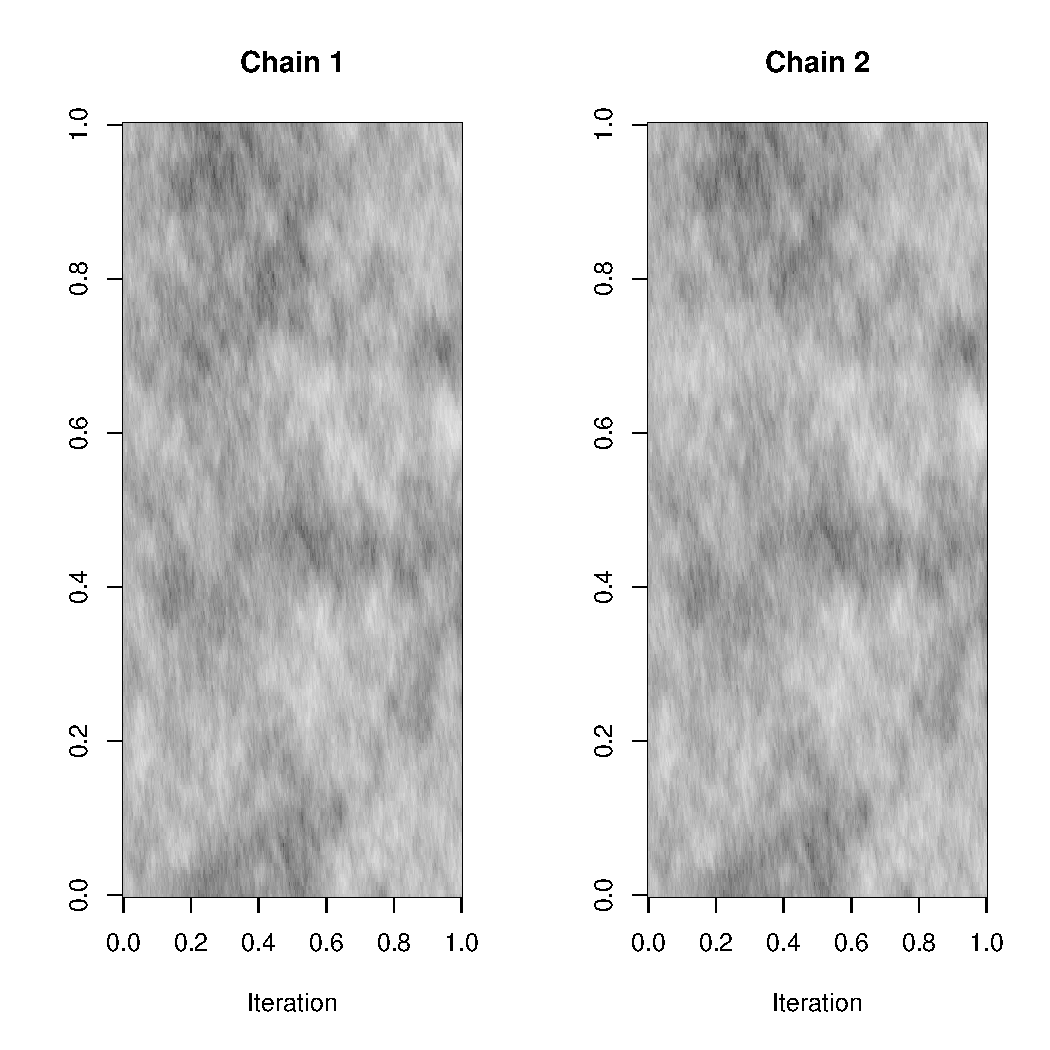
\includegraphics[height=5cm]{figs/coupled-chains}
    \qquad
    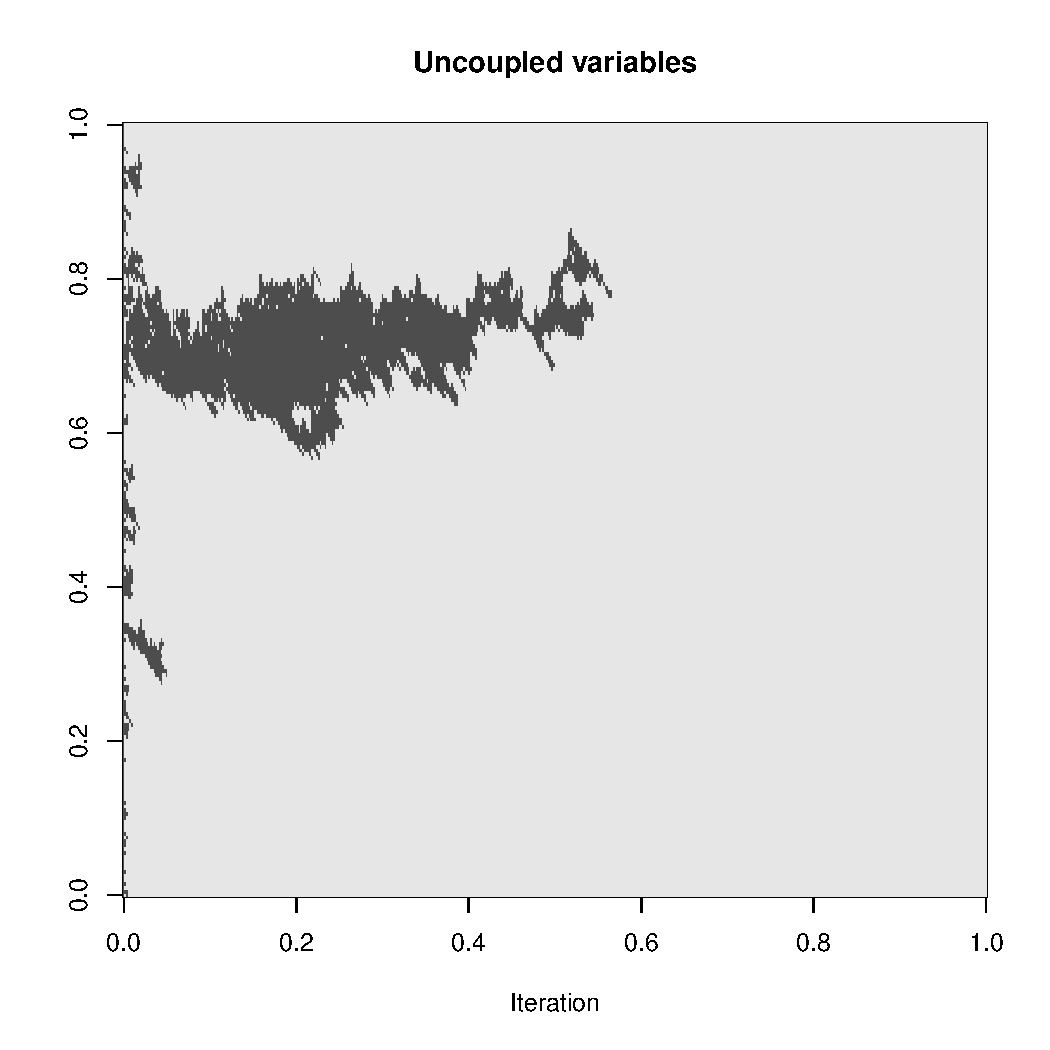
\includegraphics[height=5cm]{figs/uncoupled}
    \qquad
  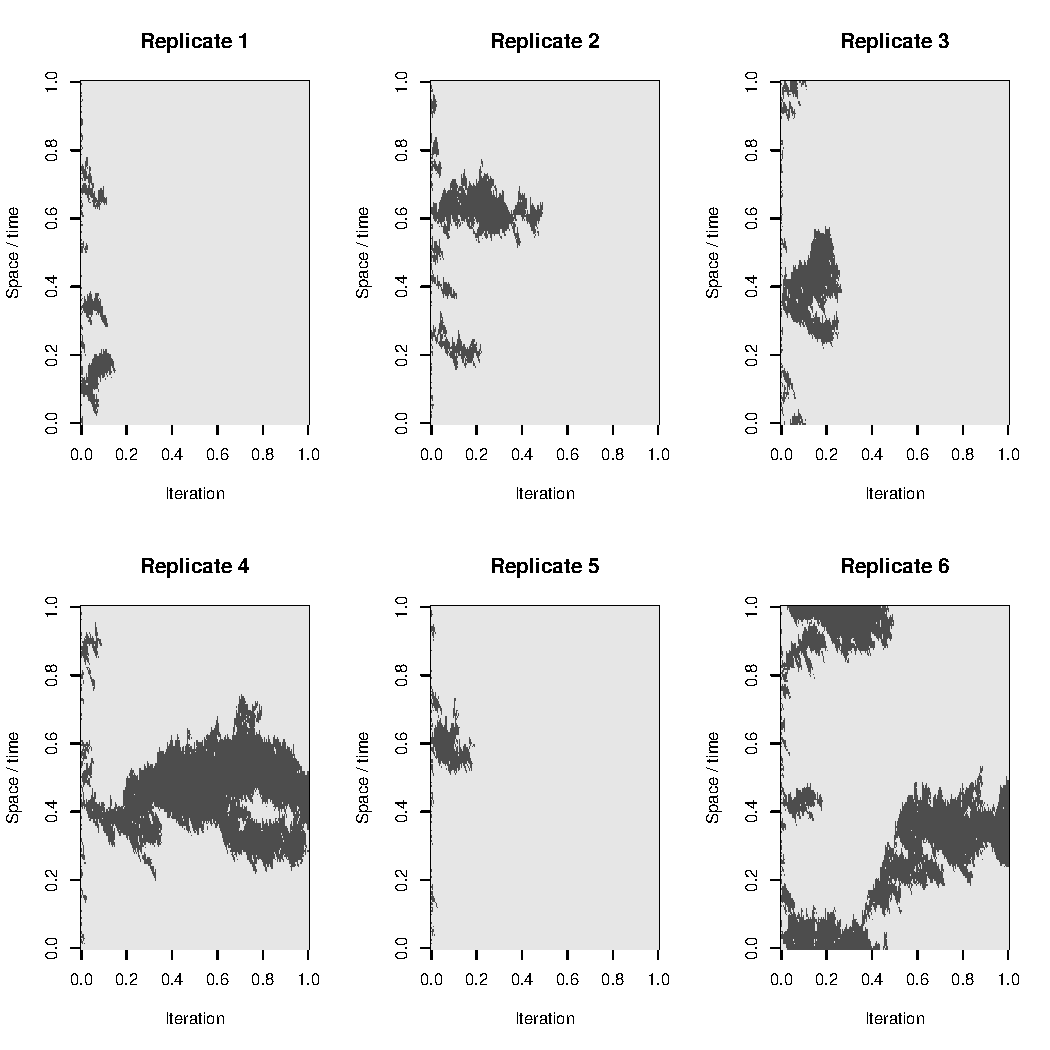
\includegraphics[height=5cm]{figs/uncoupled6}
  }
\caption{Coupled AR(1) chains (left) and a plot showing the uncoupled AR(1) variables (middle) and for six additional replicates (right). Two of these six replicates failed to coalesce within 500 iterations.}
\end{figure}

One of the main motivations for obtaining unbiased estimates of posterior expectations is to fix one of the issues with parallel chains MCMC.
We would like to run many chains independently on different processors and then pool results in some way.
In this case any bias in the chains will not ``average out'' across multiple processors, since there will be non-negligible bias in every chain.
Unbiased estimators can be safely averaged to get new unbiased estimators with reduced variance.
However, the debiasing doesn't actually eliminate burn-in --- it just corrects for it, so there is still repeated burn-in, limiting the scalability of the parallel chains approach. The paper recommends choosing $k$ as a high quantile of the coupling time distribution, and $m$ a multiple of~$k$. Any non-zero $k$ limits speed-up of parallel coupled chains relative to one long run, via \emph{Amdahl's law} for parallel chains MCMC (Wilkinson, 2005):
    \[
\text{SpeedUp}(N) = \frac{b+n}{b+\frac{n}{N}} \overset{N}{\underset{\infty}{\longrightarrow}} \frac{b+n}{b},
    \]
    for burn-in $b$ and monitoring run $n$ on $N$ processors (eg. asymptotic limit of 10 for $n=9b$). This suggests that parallel chains may be useful in the context of a small number of available processors ($\sim 10^1$), but possibly an increasingly inefficient proposition for large numbers of processors ($>\sim 10^{2}$).

 The method proposed in the paper is often straightforward to implement and seems to work on a broad range of samplers.
It is potentially useful in the context of parallelisation of MCMC algorithms, since averaging unbiased estimators is relatively safe, but it is not clear that it fundamentally solves parallel MCMC, since some kind of burn-in must still be repeated for every pair of chains.
Many open questions remain regarding the co-development of MCMC and coupling algorithms for overall efficiency.
Overall, this represents an interesting and thought-provoking contribution to the literature, and so it gives me great pleasure to propose the vote of thanks.

  \subsection*{References}

  \begin{description}
\item Wilkinson, D. J. (2005) Parallel Bayesian Computation, Chapter 16 in E. J. Kontoghiorghes (ed.) Handbook of Parallel Computing and Statistics, Marcel Dekker/CRC Press, 481-512.
    \end{description}
  

\end{document}
